\documentclass{article} % For LaTeX2e
\usepackage{iclr2022_conference,times}
% Optional math commands from https://github.com/goodfeli/dlbook_notation.
%%%%% NEW MATH DEFINITIONS %%%%%

\usepackage{amsmath,amsfonts,bm}

% Mark sections of captions for referring to divisions of figures
\newcommand{\figleft}{{\em (Left)}}
\newcommand{\figcenter}{{\em (Center)}}
\newcommand{\figright}{{\em (Right)}}
\newcommand{\figtop}{{\em (Top)}}
\newcommand{\figbottom}{{\em (Bottom)}}
\newcommand{\captiona}{{\em (a)}}
\newcommand{\captionb}{{\em (b)}}
\newcommand{\captionc}{{\em (c)}}
\newcommand{\captiond}{{\em (d)}}

% Highlight a newly defined term
\newcommand{\newterm}[1]{{\bf #1}}


% Figure reference, lower-case.
\def\figref#1{figure~\ref{#1}}
% Figure reference, capital. For start of sentence
\def\Figref#1{Figure~\ref{#1}}
\def\twofigref#1#2{figures \ref{#1} and \ref{#2}}
\def\quadfigref#1#2#3#4{figures \ref{#1}, \ref{#2}, \ref{#3} and \ref{#4}}
% Section reference, lower-case.
\def\secref#1{section~\ref{#1}}
% Section reference, capital.
\def\Secref#1{Section~\ref{#1}}
% Reference to two sections.
\def\twosecrefs#1#2{sections \ref{#1} and \ref{#2}}
% Reference to three sections.
\def\secrefs#1#2#3{sections \ref{#1}, \ref{#2} and \ref{#3}}
% Reference to an equation, lower-case.
\def\eqref#1{equation~\ref{#1}}
% Reference to an equation, upper case
\def\Eqref#1{Equation~\ref{#1}}
% A raw reference to an equation---avoid using if possible
\def\plaineqref#1{\ref{#1}}
% Reference to a chapter, lower-case.
\def\chapref#1{chapter~\ref{#1}}
% Reference to an equation, upper case.
\def\Chapref#1{Chapter~\ref{#1}}
% Reference to a range of chapters
\def\rangechapref#1#2{chapters\ref{#1}--\ref{#2}}
% Reference to an algorithm, lower-case.
\def\algref#1{algorithm~\ref{#1}}
% Reference to an algorithm, upper case.
\def\Algref#1{Algorithm~\ref{#1}}
\def\twoalgref#1#2{algorithms \ref{#1} and \ref{#2}}
\def\Twoalgref#1#2{Algorithms \ref{#1} and \ref{#2}}
% Reference to a part, lower case
\def\partref#1{part~\ref{#1}}
% Reference to a part, upper case
\def\Partref#1{Part~\ref{#1}}
\def\twopartref#1#2{parts \ref{#1} and \ref{#2}}

\def\ceil#1{\lceil #1 \rceil}
\def\floor#1{\lfloor #1 \rfloor}
\def\1{\bm{1}}
\newcommand{\train}{\mathcal{D}}
\newcommand{\valid}{\mathcal{D_{\mathrm{valid}}}}
\newcommand{\test}{\mathcal{D_{\mathrm{test}}}}

\def\eps{{\epsilon}}


% Random variables
\def\reta{{\textnormal{$\eta$}}}
\def\ra{{\textnormal{a}}}
\def\rb{{\textnormal{b}}}
\def\rc{{\textnormal{c}}}
\def\rd{{\textnormal{d}}}
\def\re{{\textnormal{e}}}
\def\rf{{\textnormal{f}}}
\def\rg{{\textnormal{g}}}
\def\rh{{\textnormal{h}}}
\def\ri{{\textnormal{i}}}
\def\rj{{\textnormal{j}}}
\def\rk{{\textnormal{k}}}
\def\rl{{\textnormal{l}}}
% rm is already a command, just don't name any random variables m
\def\rn{{\textnormal{n}}}
\def\ro{{\textnormal{o}}}
\def\rp{{\textnormal{p}}}
\def\rq{{\textnormal{q}}}
\def\rr{{\textnormal{r}}}
\def\rs{{\textnormal{s}}}
\def\rt{{\textnormal{t}}}
\def\ru{{\textnormal{u}}}
\def\rv{{\textnormal{v}}}
\def\rw{{\textnormal{w}}}
\def\rx{{\textnormal{x}}}
\def\ry{{\textnormal{y}}}
\def\rz{{\textnormal{z}}}

% Random vectors
\def\rvepsilon{{\mathbf{\epsilon}}}
\def\rvtheta{{\mathbf{\theta}}}
\def\rva{{\mathbf{a}}}
\def\rvb{{\mathbf{b}}}
\def\rvc{{\mathbf{c}}}
\def\rvd{{\mathbf{d}}}
\def\rve{{\mathbf{e}}}
\def\rvf{{\mathbf{f}}}
\def\rvg{{\mathbf{g}}}
\def\rvh{{\mathbf{h}}}
\def\rvu{{\mathbf{i}}}
\def\rvj{{\mathbf{j}}}
\def\rvk{{\mathbf{k}}}
\def\rvl{{\mathbf{l}}}
\def\rvm{{\mathbf{m}}}
\def\rvn{{\mathbf{n}}}
\def\rvo{{\mathbf{o}}}
\def\rvp{{\mathbf{p}}}
\def\rvq{{\mathbf{q}}}
\def\rvr{{\mathbf{r}}}
\def\rvs{{\mathbf{s}}}
\def\rvt{{\mathbf{t}}}
\def\rvu{{\mathbf{u}}}
\def\rvv{{\mathbf{v}}}
\def\rvw{{\mathbf{w}}}
\def\rvx{{\mathbf{x}}}
\def\rvy{{\mathbf{y}}}
\def\rvz{{\mathbf{z}}}

% Elements of random vectors
\def\erva{{\textnormal{a}}}
\def\ervb{{\textnormal{b}}}
\def\ervc{{\textnormal{c}}}
\def\ervd{{\textnormal{d}}}
\def\erve{{\textnormal{e}}}
\def\ervf{{\textnormal{f}}}
\def\ervg{{\textnormal{g}}}
\def\ervh{{\textnormal{h}}}
\def\ervi{{\textnormal{i}}}
\def\ervj{{\textnormal{j}}}
\def\ervk{{\textnormal{k}}}
\def\ervl{{\textnormal{l}}}
\def\ervm{{\textnormal{m}}}
\def\ervn{{\textnormal{n}}}
\def\ervo{{\textnormal{o}}}
\def\ervp{{\textnormal{p}}}
\def\ervq{{\textnormal{q}}}
\def\ervr{{\textnormal{r}}}
\def\ervs{{\textnormal{s}}}
\def\ervt{{\textnormal{t}}}
\def\ervu{{\textnormal{u}}}
\def\ervv{{\textnormal{v}}}
\def\ervw{{\textnormal{w}}}
\def\ervx{{\textnormal{x}}}
\def\ervy{{\textnormal{y}}}
\def\ervz{{\textnormal{z}}}

% Random matrices
\def\rmA{{\mathbf{A}}}
\def\rmB{{\mathbf{B}}}
\def\rmC{{\mathbf{C}}}
\def\rmD{{\mathbf{D}}}
\def\rmE{{\mathbf{E}}}
\def\rmF{{\mathbf{F}}}
\def\rmG{{\mathbf{G}}}
\def\rmH{{\mathbf{H}}}
\def\rmI{{\mathbf{I}}}
\def\rmJ{{\mathbf{J}}}
\def\rmK{{\mathbf{K}}}
\def\rmL{{\mathbf{L}}}
\def\rmM{{\mathbf{M}}}
\def\rmN{{\mathbf{N}}}
\def\rmO{{\mathbf{O}}}
\def\rmP{{\mathbf{P}}}
\def\rmQ{{\mathbf{Q}}}
\def\rmR{{\mathbf{R}}}
\def\rmS{{\mathbf{S}}}
\def\rmT{{\mathbf{T}}}
\def\rmU{{\mathbf{U}}}
\def\rmV{{\mathbf{V}}}
\def\rmW{{\mathbf{W}}}
\def\rmX{{\mathbf{X}}}
\def\rmY{{\mathbf{Y}}}
\def\rmZ{{\mathbf{Z}}}

% Elements of random matrices
\def\ermA{{\textnormal{A}}}
\def\ermB{{\textnormal{B}}}
\def\ermC{{\textnormal{C}}}
\def\ermD{{\textnormal{D}}}
\def\ermE{{\textnormal{E}}}
\def\ermF{{\textnormal{F}}}
\def\ermG{{\textnormal{G}}}
\def\ermH{{\textnormal{H}}}
\def\ermI{{\textnormal{I}}}
\def\ermJ{{\textnormal{J}}}
\def\ermK{{\textnormal{K}}}
\def\ermL{{\textnormal{L}}}
\def\ermM{{\textnormal{M}}}
\def\ermN{{\textnormal{N}}}
\def\ermO{{\textnormal{O}}}
\def\ermP{{\textnormal{P}}}
\def\ermQ{{\textnormal{Q}}}
\def\ermR{{\textnormal{R}}}
\def\ermS{{\textnormal{S}}}
\def\ermT{{\textnormal{T}}}
\def\ermU{{\textnormal{U}}}
\def\ermV{{\textnormal{V}}}
\def\ermW{{\textnormal{W}}}
\def\ermX{{\textnormal{X}}}
\def\ermY{{\textnormal{Y}}}
\def\ermZ{{\textnormal{Z}}}

% Vectors
\def\vzero{{\bm{0}}}
\def\vone{{\bm{1}}}
\def\vmu{{\bm{\mu}}}
\def\vtheta{{\bm{\theta}}}
\def\va{{\bm{a}}}
\def\vb{{\bm{b}}}
\def\vc{{\bm{c}}}
\def\vd{{\bm{d}}}
\def\ve{{\bm{e}}}
\def\vf{{\bm{f}}}
\def\vg{{\bm{g}}}
\def\vh{{\bm{h}}}
\def\vi{{\bm{i}}}
\def\vj{{\bm{j}}}
\def\vk{{\bm{k}}}
\def\vl{{\bm{l}}}
\def\vm{{\bm{m}}}
\def\vn{{\bm{n}}}
\def\vo{{\bm{o}}}
\def\vp{{\bm{p}}}
\def\vq{{\bm{q}}}
\def\vr{{\bm{r}}}
\def\vs{{\bm{s}}}
\def\vt{{\bm{t}}}
\def\vu{{\bm{u}}}
\def\vv{{\bm{v}}}
\def\vw{{\bm{w}}}
\def\vx{{\bm{x}}}
\def\vy{{\bm{y}}}
\def\vz{{\bm{z}}}

% Elements of vectors
\def\evalpha{{\alpha}}
\def\evbeta{{\beta}}
\def\evepsilon{{\epsilon}}
\def\evlambda{{\lambda}}
\def\evomega{{\omega}}
\def\evmu{{\mu}}
\def\evpsi{{\psi}}
\def\evsigma{{\sigma}}
\def\evtheta{{\theta}}
\def\eva{{a}}
\def\evb{{b}}
\def\evc{{c}}
\def\evd{{d}}
\def\eve{{e}}
\def\evf{{f}}
\def\evg{{g}}
\def\evh{{h}}
\def\evi{{i}}
\def\evj{{j}}
\def\evk{{k}}
\def\evl{{l}}
\def\evm{{m}}
\def\evn{{n}}
\def\evo{{o}}
\def\evp{{p}}
\def\evq{{q}}
\def\evr{{r}}
\def\evs{{s}}
\def\evt{{t}}
\def\evu{{u}}
\def\evv{{v}}
\def\evw{{w}}
\def\evx{{x}}
\def\evy{{y}}
\def\evz{{z}}

% Matrix
\def\mA{{\bm{A}}}
\def\mB{{\bm{B}}}
\def\mC{{\bm{C}}}
\def\mD{{\bm{D}}}
\def\mE{{\bm{E}}}
\def\mF{{\bm{F}}}
\def\mG{{\bm{G}}}
\def\mH{{\bm{H}}}
\def\mI{{\bm{I}}}
\def\mJ{{\bm{J}}}
\def\mK{{\bm{K}}}
\def\mL{{\bm{L}}}
\def\mM{{\bm{M}}}
\def\mN{{\bm{N}}}
\def\mO{{\bm{O}}}
\def\mP{{\bm{P}}}
\def\mQ{{\bm{Q}}}
\def\mR{{\bm{R}}}
\def\mS{{\bm{S}}}
\def\mT{{\bm{T}}}
\def\mU{{\bm{U}}}
\def\mV{{\bm{V}}}
\def\mW{{\bm{W}}}
\def\mX{{\bm{X}}}
\def\mY{{\bm{Y}}}
\def\mZ{{\bm{Z}}}
\def\mBeta{{\bm{\beta}}}
\def\mPhi{{\bm{\Phi}}}
\def\mLambda{{\bm{\Lambda}}}
\def\mSigma{{\bm{\Sigma}}}

% Tensor
\DeclareMathAlphabet{\mathsfit}{\encodingdefault}{\sfdefault}{m}{sl}
\SetMathAlphabet{\mathsfit}{bold}{\encodingdefault}{\sfdefault}{bx}{n}
\newcommand{\tens}[1]{\bm{\mathsfit{#1}}}
\def\tA{{\tens{A}}}
\def\tB{{\tens{B}}}
\def\tC{{\tens{C}}}
\def\tD{{\tens{D}}}
\def\tE{{\tens{E}}}
\def\tF{{\tens{F}}}
\def\tG{{\tens{G}}}
\def\tH{{\tens{H}}}
\def\tI{{\tens{I}}}
\def\tJ{{\tens{J}}}
\def\tK{{\tens{K}}}
\def\tL{{\tens{L}}}
\def\tM{{\tens{M}}}
\def\tN{{\tens{N}}}
\def\tO{{\tens{O}}}
\def\tP{{\tens{P}}}
\def\tQ{{\tens{Q}}}
\def\tR{{\tens{R}}}
\def\tS{{\tens{S}}}
\def\tT{{\tens{T}}}
\def\tU{{\tens{U}}}
\def\tV{{\tens{V}}}
\def\tW{{\tens{W}}}
\def\tX{{\tens{X}}}
\def\tY{{\tens{Y}}}
\def\tZ{{\tens{Z}}}


% Graph
\def\gA{{\mathcal{A}}}
\def\gB{{\mathcal{B}}}
\def\gC{{\mathcal{C}}}
\def\gD{{\mathcal{D}}}
\def\gE{{\mathcal{E}}}
\def\gF{{\mathcal{F}}}
\def\gG{{\mathcal{G}}}
\def\gH{{\mathcal{H}}}
\def\gI{{\mathcal{I}}}
\def\gJ{{\mathcal{J}}}
\def\gK{{\mathcal{K}}}
\def\gL{{\mathcal{L}}}
\def\gM{{\mathcal{M}}}
\def\gN{{\mathcal{N}}}
\def\gO{{\mathcal{O}}}
\def\gP{{\mathcal{P}}}
\def\gQ{{\mathcal{Q}}}
\def\gR{{\mathcal{R}}}
\def\gS{{\mathcal{S}}}
\def\gT{{\mathcal{T}}}
\def\gU{{\mathcal{U}}}
\def\gV{{\mathcal{V}}}
\def\gW{{\mathcal{W}}}
\def\gX{{\mathcal{X}}}
\def\gY{{\mathcal{Y}}}
\def\gZ{{\mathcal{Z}}}

% Sets
\def\sA{{\mathbb{A}}}
\def\sB{{\mathbb{B}}}
\def\sC{{\mathbb{C}}}
\def\sD{{\mathbb{D}}}
% Don't use a set called E, because this would be the same as our symbol
% for expectation.
\def\sF{{\mathbb{F}}}
\def\sG{{\mathbb{G}}}
\def\sH{{\mathbb{H}}}
\def\sI{{\mathbb{I}}}
\def\sJ{{\mathbb{J}}}
\def\sK{{\mathbb{K}}}
\def\sL{{\mathbb{L}}}
\def\sM{{\mathbb{M}}}
\def\sN{{\mathbb{N}}}
\def\sO{{\mathbb{O}}}
\def\sP{{\mathbb{P}}}
\def\sQ{{\mathbb{Q}}}
\def\sR{{\mathbb{R}}}
\def\sS{{\mathbb{S}}}
\def\sT{{\mathbb{T}}}
\def\sU{{\mathbb{U}}}
\def\sV{{\mathbb{V}}}
\def\sW{{\mathbb{W}}}
\def\sX{{\mathbb{X}}}
\def\sY{{\mathbb{Y}}}
\def\sZ{{\mathbb{Z}}}

% Entries of a matrix
\def\emLambda{{\Lambda}}
\def\emA{{A}}
\def\emB{{B}}
\def\emC{{C}}
\def\emD{{D}}
\def\emE{{E}}
\def\emF{{F}}
\def\emG{{G}}
\def\emH{{H}}
\def\emI{{I}}
\def\emJ{{J}}
\def\emK{{K}}
\def\emL{{L}}
\def\emM{{M}}
\def\emN{{N}}
\def\emO{{O}}
\def\emP{{P}}
\def\emQ{{Q}}
\def\emR{{R}}
\def\emS{{S}}
\def\emT{{T}}
\def\emU{{U}}
\def\emV{{V}}
\def\emW{{W}}
\def\emX{{X}}
\def\emY{{Y}}
\def\emZ{{Z}}
\def\emSigma{{\Sigma}}

% entries of a tensor
% Same font as tensor, without \bm wrapper
\newcommand{\etens}[1]{\mathsfit{#1}}
\def\etLambda{{\etens{\Lambda}}}
\def\etA{{\etens{A}}}
\def\etB{{\etens{B}}}
\def\etC{{\etens{C}}}
\def\etD{{\etens{D}}}
\def\etE{{\etens{E}}}
\def\etF{{\etens{F}}}
\def\etG{{\etens{G}}}
\def\etH{{\etens{H}}}
\def\etI{{\etens{I}}}
\def\etJ{{\etens{J}}}
\def\etK{{\etens{K}}}
\def\etL{{\etens{L}}}
\def\etM{{\etens{M}}}
\def\etN{{\etens{N}}}
\def\etO{{\etens{O}}}
\def\etP{{\etens{P}}}
\def\etQ{{\etens{Q}}}
\def\etR{{\etens{R}}}
\def\etS{{\etens{S}}}
\def\etT{{\etens{T}}}
\def\etU{{\etens{U}}}
\def\etV{{\etens{V}}}
\def\etW{{\etens{W}}}
\def\etX{{\etens{X}}}
\def\etY{{\etens{Y}}}
\def\etZ{{\etens{Z}}}

% The true underlying data generating distribution
\newcommand{\pdata}{p_{\rm{data}}}
% The empirical distribution defined by the training set
\newcommand{\ptrain}{\hat{p}_{\rm{data}}}
\newcommand{\Ptrain}{\hat{P}_{\rm{data}}}
% The model distribution
\newcommand{\pmodel}{p_{\rm{model}}}
\newcommand{\Pmodel}{P_{\rm{model}}}
\newcommand{\ptildemodel}{\tilde{p}_{\rm{model}}}
% Stochastic autoencoder distributions
\newcommand{\pencode}{p_{\rm{encoder}}}
\newcommand{\pdecode}{p_{\rm{decoder}}}
\newcommand{\precons}{p_{\rm{reconstruct}}}

\newcommand{\laplace}{\mathrm{Laplace}} % Laplace distribution

\newcommand{\E}{\mathbb{E}}
\newcommand{\Ls}{\mathcal{L}}
\newcommand{\R}{\mathbb{R}}
\newcommand{\emp}{\tilde{p}}
\newcommand{\lr}{\alpha}
\newcommand{\reg}{\lambda}
\newcommand{\rect}{\mathrm{rectifier}}
\newcommand{\softmax}{\mathrm{softmax}}
\newcommand{\sigmoid}{\sigma}
\newcommand{\softplus}{\zeta}
\newcommand{\KL}{D_{\mathrm{KL}}}
\newcommand{\Var}{\mathrm{Var}}
\newcommand{\standarderror}{\mathrm{SE}}
\newcommand{\Cov}{\mathrm{Cov}}
% Wolfram Mathworld says $L^2$ is for function spaces and $\ell^2$ is for vectors
% But then they seem to use $L^2$ for vectors throughout the site, and so does
% wikipedia.
\newcommand{\normlzero}{L^0}
\newcommand{\normlone}{L^1}
\newcommand{\normltwo}{L^2}
\newcommand{\normlp}{L^p}
\newcommand{\normmax}{L^\infty}

\newcommand{\parents}{Pa} % See usage in notation.tex. Chosen to match Daphne's book.

\DeclareMathOperator*{\argmax}{arg\,max}
\DeclareMathOperator*{\argmin}{arg\,min}

\DeclareMathOperator{\sign}{sign}
\DeclareMathOperator{\Tr}{Tr}
\let\ab\allowbreak


%######## APS360: Uncomment your submission name
%\newcommand{\apsname}{Project Proposal}
%\newcommand{\apsname}{Progress Report}
\newcommand{\apsname}{Final Report}

%######## APS360: Put your Group Number here
\newcommand{\gpnumber}{20}

\usepackage{hyperref}
\usepackage{url}
\usepackage{graphicx}
\usepackage{multicol}

%######## APS360: Put your project Title here
\title{Poetry Through Propogation,\ Generating Haikus With Deep Learning Recurrent Neural Networks}


%######## APS360: Put your names, student IDs and Emails here
\author{Evan Banerjee  \\
Student\# 1009682309\\
\texttt{evan.banerjee@mail.utoronto.ca} \\
\And
Diego Ciudad Real Escalante  \\
Student\# 1009345308 \\
\texttt{diego.ciudadrealescalante@mail.utoronto.ca} \\
\AND
Noah Monti  \\
Student\# 1009452398 \\
\texttt{noah.monti@mail.utoronto.ca} \\
\And
Ji Hong Sayo \\
Student\# 1007314728 \\
\texttt{ji.sayo@mail.utoronto.ca} \\
\AND
}

% The \author macro works with any number of authors. There are two commands
% used to separate the names and addresses of multiple authors: \And and \AND.
%
% Using \And between authors leaves it to \LaTeX{} to determine where to break
% the lines. Using \AND forces a linebreak at that point. So, if \LaTeX{}
% puts 3 of 4 authors names on the first line, and the last on the second
% line, try using \AND instead of \And before the third author name.

\newcommand{\fix}{\marginpar{FIX}}
\newcommand{\new}{\marginpar{NEW}}

\iclrfinalcopy 
%######## APS360: Document starts here
\begin{document}


\maketitle

\begin{abstract}
This is our progress report for the APS360 Final Project.
%######## APS360: Do not change the next line. This shows your Main body page count.
Total Pages: \pageref{last_page}
\end{abstract}

\section{Introduction}

\section{Illustriaton}

% \begin{figure}[h]
%   \begin{center}
%   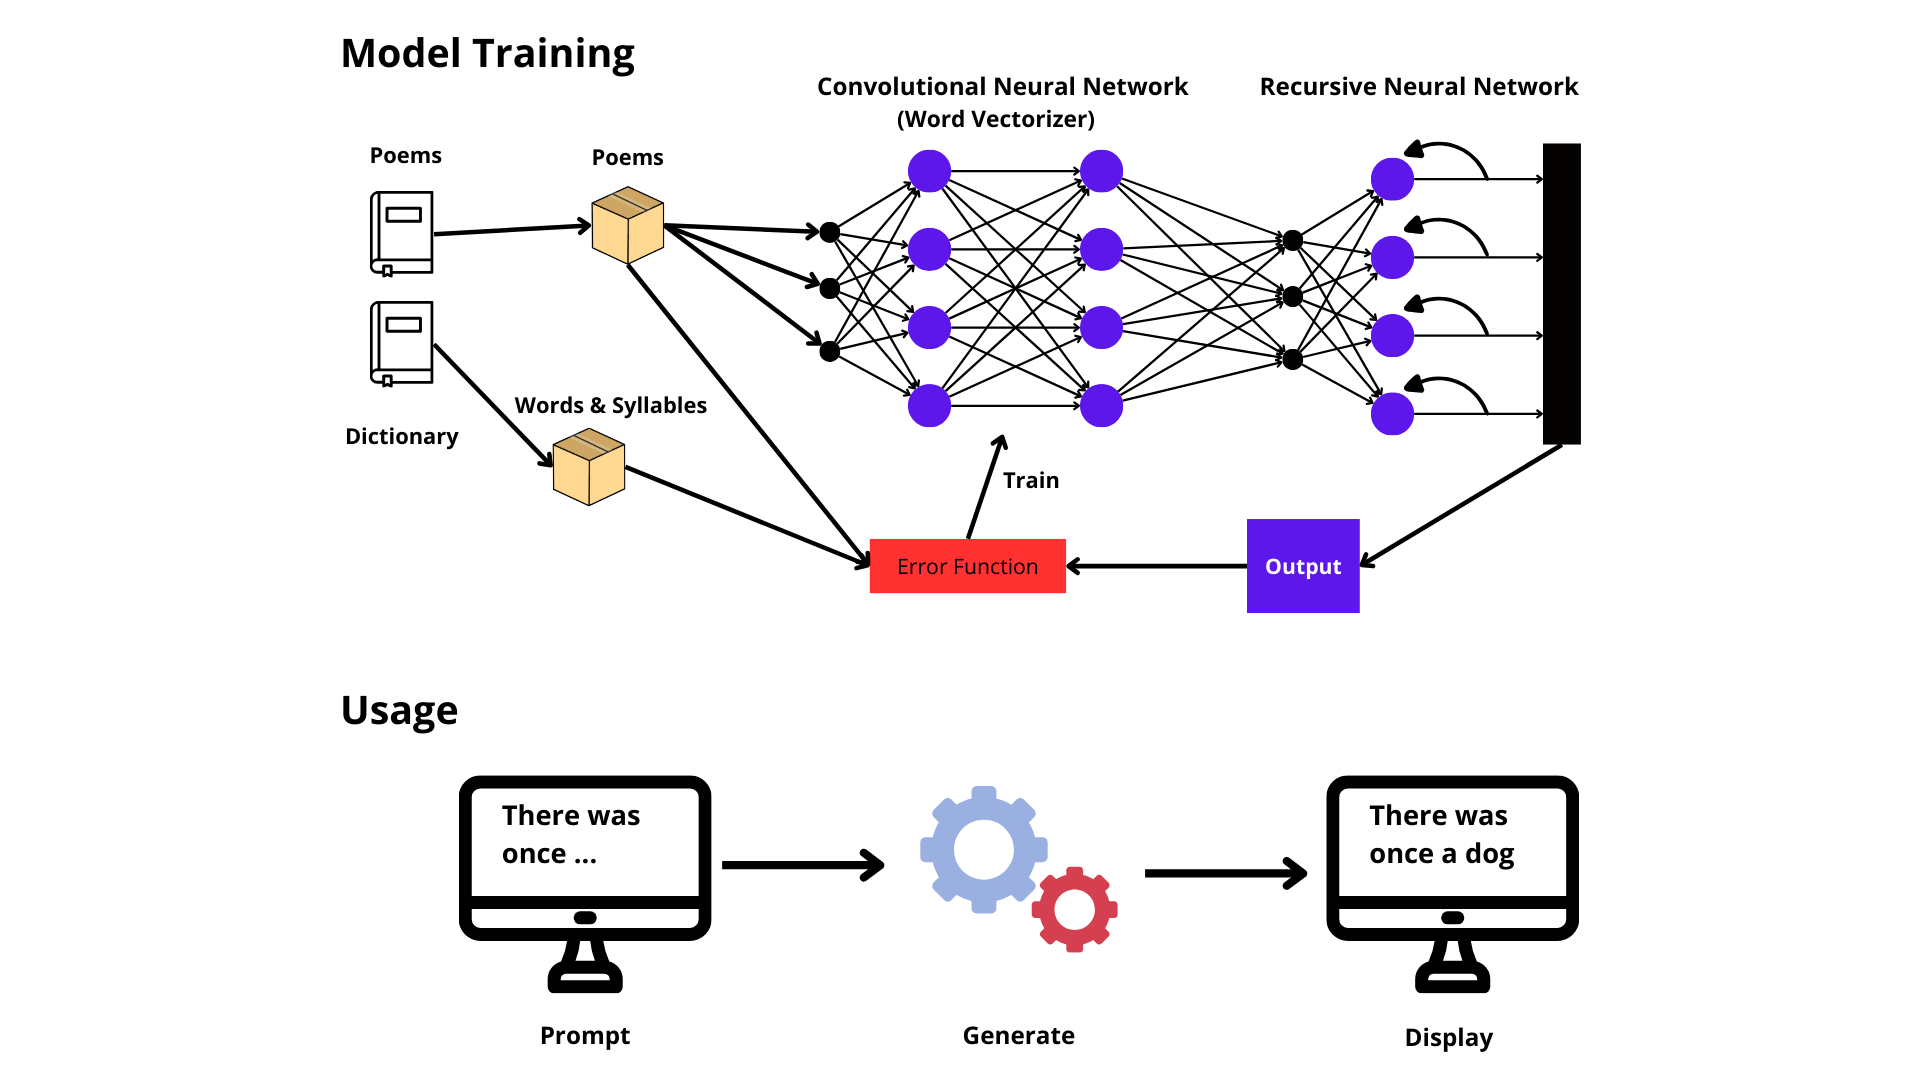
\includegraphics[width=1\textwidth]{Figs/model_diagram.png}
%   \end{center}
%   \caption{Basic Model Pipeline}
%   \label{fig:pipeline}
% \end{figure}

\section{Background}

\section{Project Description}

Project Description
“Genuine poetry can communicate before it is understood” —T.S. Eliot
In this project we are working to build a deep learning model to generate short poems of various topics.
Our model is a haiku generator which can be prompted with the first line of a haiku and generate the content of subsequent lines, built on an LSTM (long-short-term-memory) architecture.
Poetry has long been regarded as a deep expression of emotion and human experience. Given that the model we construct will possess neither emotions nor intuition, we are interested to see whether our construction will be able to imitate human poetry, and if so to what degree. If the model is capable of producing compelling poems as output, this would contradict the idea that poetry requires emotion to produce, with implications for our understanding of the nature of creative work in general.

% \begin{figure}[h]
%   \begin{center}
%   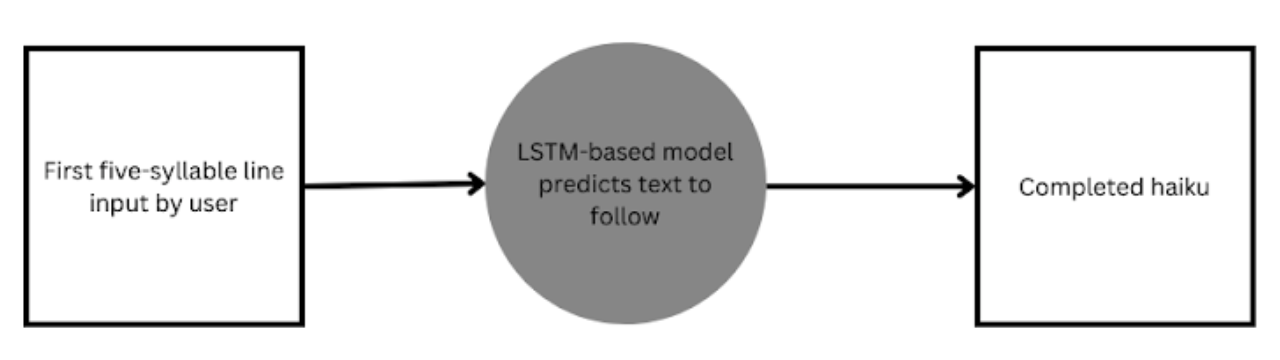
\includegraphics[width=1\textwidth]{Figs/pipeline.png}
%   \end{center}
%   \caption{Basic Model Pipeline}
%   \label{fig:pipeline}
% \end{figure}

Several ML approaches can be taken to text-generation.
For instance, we compare our model to markov chains as a baseline.
However, deep learning offers advantages that other statistical approaches cannot.
As compared to simpler statistical models, neural nets can learn more abstract and general characteristics in the poems used for training.
Given that a hallmark of good poetry is abstraction and unity around a sustaining theme,
we believe deep learning is uniquely well-suited for the problem of poetry generation.

\section{Individual Contributions and Responsibilities}

Thus far our team has been performing effectively—we have been able to meet both internal and external deadlines. Currently, we've been collaborating over github, with most team members working in jupyter notebooks we upload to the shared github page for review. Team communication takes place over whatsapp, and both systems have been working well thus far.

On a technical level, we are quite pleased with our progress thus far, which has been facilitated by the fact that training on text is less memory-intensive than training on images, which allows for more rapid prototyping without consuming very large amounts of computing power. We have already implemented both 'baseline' and prototype models. What remains is hyperparameter tuning, improvements to the model and testing, all of which we feel will be completed well within the timeframe of the project. In summary, we are on track to meet the goals outlined in our proposal, and may even implement some additional testing and functionality beyond what was outlined in our initial proposal.


\subsection{Redundancies}

The most crucial remaining aspect of our project is training the finalized model with a consolidated dataset. This is also a potentially sensitive step, as connection losses or malfunctions could result in significant investments of time and computational resources being wasted. Given this, we plan to have two team members responsible for training. If the primary team member runs into difficulties, they will quickly alert the team via WhatsApp, so that the secondary group member can take over and begin training on a separate system, thus reducing the risk of a technical or personal problem derailing the project.

Several of our group members have separately implemented or are working to implement different model architectures. While we have a consensus on which architecture we plan to use for the final model, this experimentation provides a strong element of redundancy. If unexpected issues emerge with the architecture we've agreed on, we can discuss as a group and fall back on one of the experimental models.

\subsection{Team Contributions and Communication}

As shown in the task tracker (Figure~\ref{fig:tasktracker}) and the communications table (Figure~\ref{fig:commstable}), all team members have been responsive and met the necessary deadlines for their work.

% \begin{figure}[h]
%   \begin{center}
%   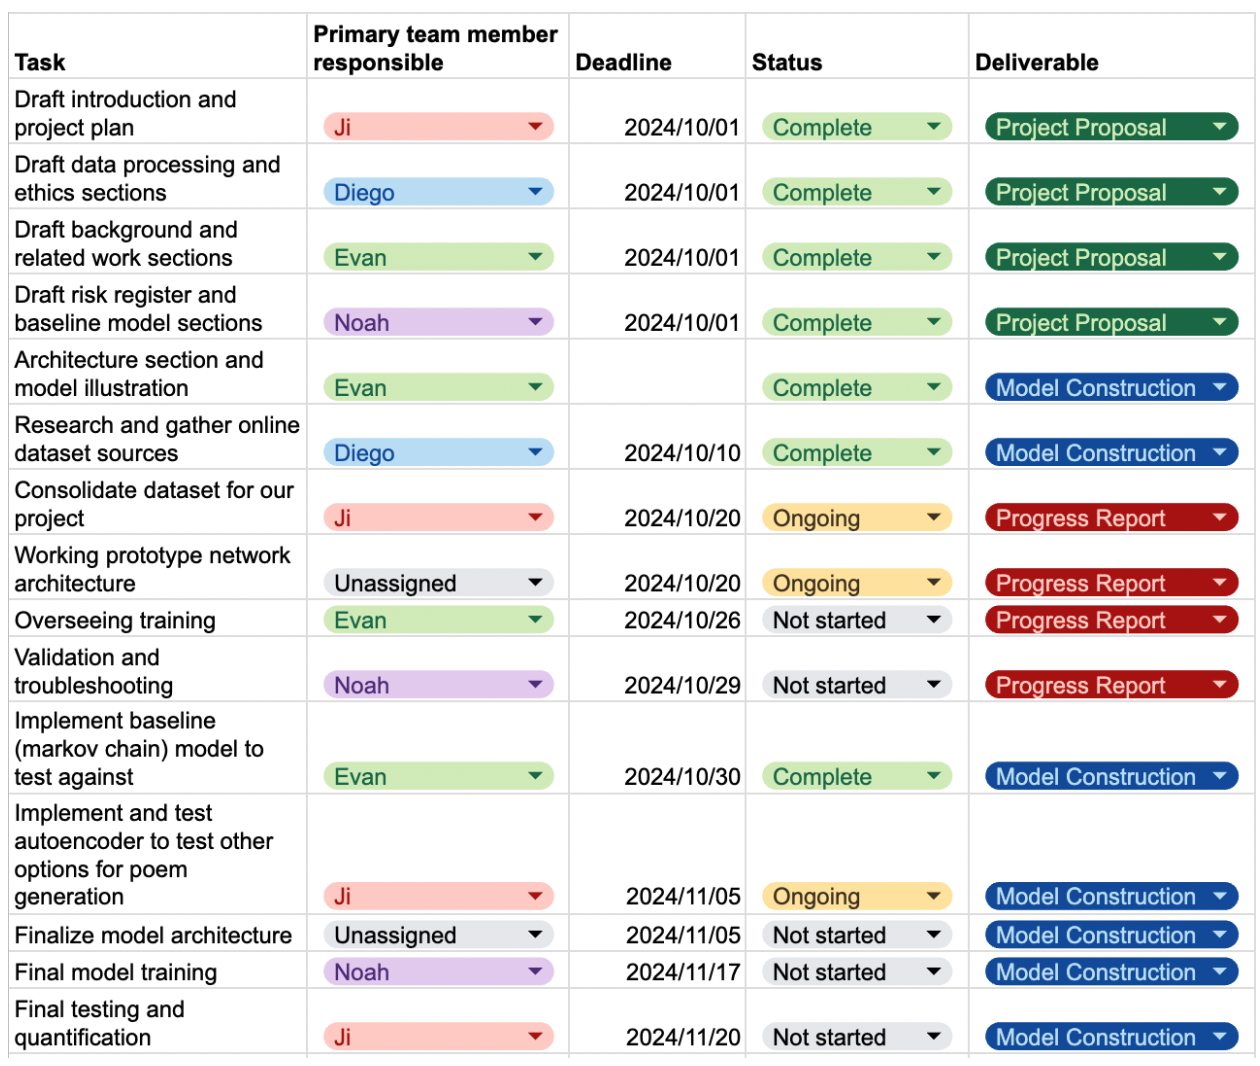
\includegraphics[width=1\textwidth]{Figs/tasktracker.png}
%   \end{center}
%   \caption{Updated Task Tracker}
%   \label{fig:tasktracker}
% \end{figure}

% \begin{figure}[h]
%   \begin{center}
%   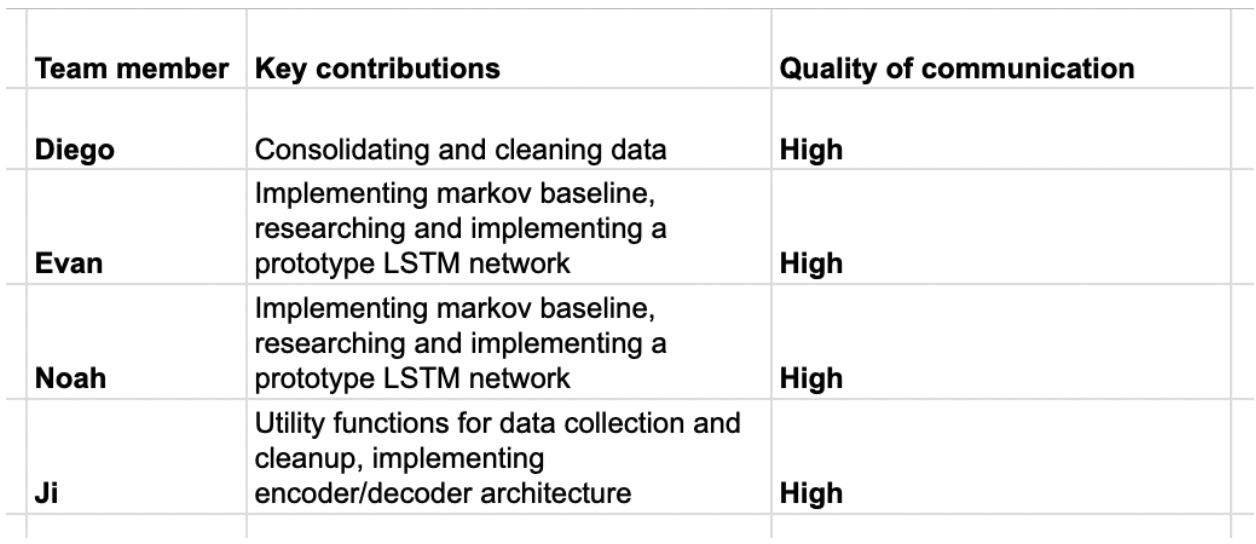
\includegraphics[width=1\textwidth]{Figs/commstable.png}
%   \end{center}
%   \caption{Team communication and contributions}
%   \label{fig:commstable}
% \end{figure}

\section{Notable Contribution}

\subsection{Data Processing}
The main data used for this project consists of the haiku4u dataset in kaggle \citep{haiku4u}.
This dataset is publicly available and comes from a web scraper run in October 2023.
The data comes in the form of a csv file which has the following fields:
Haiku, a field containing the entire haiku with lines separated by a ”$|$” character;
Domain, the name of the web page where it was originally found;
Domains, the amount of times this specific haiku was encountered while scraping the web;
URL, the specific url where the poem was found;
URLs, the number of urls that were found in in the same domain.
Siblings, the number of other Poems that were found in that same URL.
Another data source we used is the CMU pronouncing dictionary \citep{cmu_pronouncing_dictionary}.
We use this dictionary to count the amount of syllables in each line of the haiku.
Given that this is an open source project with a python library, data cleanup was minimal for this dataset.


After downloading the data, the cleaning process for the haiku dataset consists is run by a python script.
This python script takes in each row of the csv file, and removes all the rows that do not contain a haiku.
Then, it splits the haiku into its three lines based on where the $|$ delimiter can be found.
Next it converts all the characters to lowercase.
And finally, it appends the haiku to a text file in which the end of a haiku is denoted by two new line characters.
The text file is then used at training when loading the data.
Below is an example of the raw input data, and its processed form.



\begin{multicols}{2}

  \textbf{Original (Raw text):} \par
  Yesterday it worked.$|$Today it is not working.$|$Windows is
  like that.,richardneill.org,27,
  https://richardneill.org/humour.php,27,19

  \columnbreak

  \raggedleft
  \textbf{Finalized (After cleaning):} \par

  \raggedleft
  yesterday it worked.

  today it is not working.

  windows is like that.
\end{multicols}

Another use of the data is in building the vocabulary before training.
To do this we run the entirety of the text file word-by-word into a python dictionary that maps each word to an index.
This lets us represent the words encountered in a numeric form that is easier to deal with.
Finally, we must say that because the nature of this project is generative,
we testing new data simply means prompting the model differently.
However, we are actively looking into ways of increasing the training data we have access to.
Some examples of how we could do this are concatenating this data set with others like it
and scraping the web ourselves in the hopes we find many more haikus that were not seen originally in 2023.


\subsection{Baseline Model}

Our first main baseline model is a markov chain of depth four. This was trained on the same data used in the primary model.
The main structure is shown in figure 0:

\begin{figure}[h]
  \begin{center}
  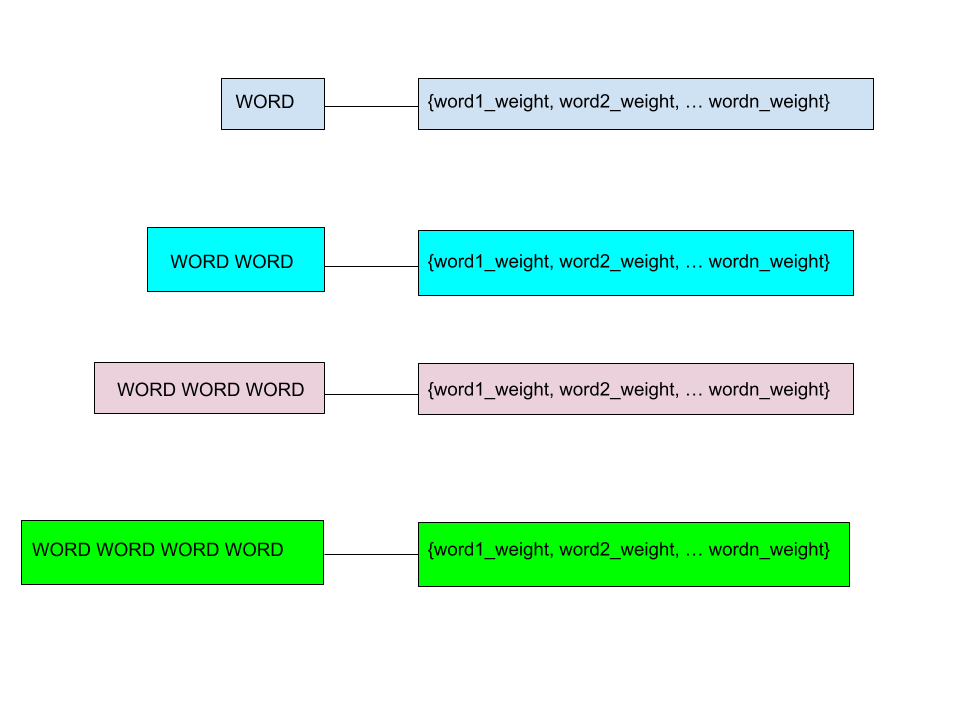
\includegraphics[width=1\textwidth]{Figs/MARKOV.png}
  \end{center}
  \caption{general weighting scheme for markov chain}
  \label{fig:plot}
  \end{figure}

Each individual word in the corpora is assigned a weighting scheme for every word (including itself) based on how frequently those other words come
after the first word.\\
Then every pair of words is assigned a weighting scheme for every word in the corpora based on how likely the word appears after the pair.\\
Then every triple of words is assigned a similar weighting scheme.\\
This repeats until you have a weighting scheme for every n-gram sequence of words up to the depth provided by the function.\\

Throughout this process we treated newline characters and "end of poem" lines (EOP) as distinct words. The model would take in a starting string of
words and would try to autocomplete the poem. It chose words by taking a weighted random choiced based on the weights calculated for the markov
datastructure\\

We chose to use a depth of 4 because lower depths had far more incoherent outputs while higher depths seemed to either return no output
or just directly copy poems for the most part. Here are some example inputs, and their corresponding outputs:\\


Show me:
\begin{flushleft}
  \textit{
      \hspace{2em} show me a garden that's \\
      \hspace{2em} bursting into life
  }
\end{flushleft}

Give:
\begin{flushleft}
  \textit{
      \hspace{2em} give your \\
      \hspace{2em} puppies a little extra\\
      \hspace{2em} thankful that god took me out\\
      \hspace{2em} this funny as hell\\
      \hspace{2em} steve's hair evolving\\
  }
\end{flushleft}


 Teach:
 \begin{flushleft}
  \textit{
      \hspace{2em} teach people  \\
      \hspace{2em} how to get folder icons\\
      \hspace{2em} to show in snowboard\\
  }
\end{flushleft}

It should be noted that these poems were hand-chosen from the markov chain for being more coherent. Often, the markov chain will simply copy
off another poem, return no output, or only return a couple of words, such as the input "teach" generating the output "teach great place to live".\\

Even in the best case, this model struggles to correctly write lines with the correct number of syllables.

We created another baseline model from a very simple LSTM RNN. the structure for this one was a much simpler version of our primary model.\\

It had a 128 dimensional embedding scheme with 2 hidden layers of dimension 256 and a learning rate of 0.001. It was trained with a batch size of 64
for 30 epochs. The output was mostly incoherent so we decided to use the Markov chain as a baseline. All the source code for the first RNN and the
Markov chain is on github, under the jupyter notebook \texttt{RNN\_Model\_1}.



\subsection{Primary Model}

The overall model architecture is described in the Figure~\ref{fig:flowchart} flowchart.

\begin{figure}[h]
  \begin{center}
  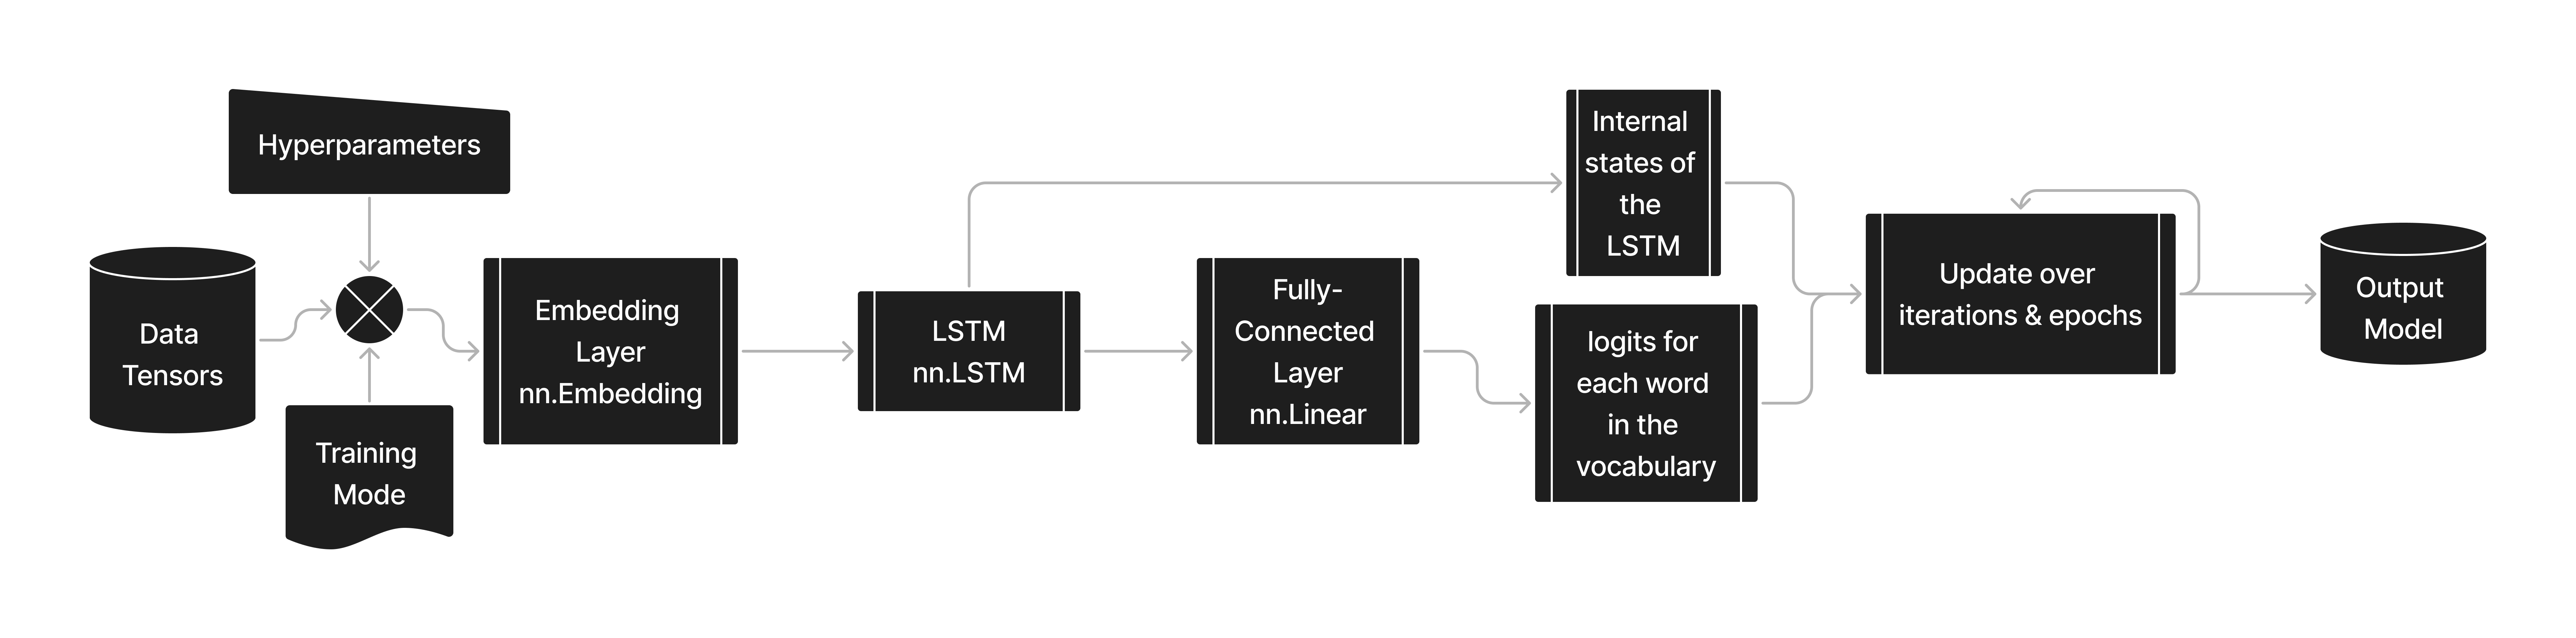
\includegraphics[width=1\textwidth]{Figs/HaikuLSTMArch.png}
  \end{center}
  \caption{Model Architecture}
  \label{fig:flowchart}
\end{figure}

For our haiku generation model, we continued with a Long Short-Term Memory (LSTM) architecture to capture the contextual nuances, and move towards generating coherent and accurate haikus.

The architecture of the model is as follows:

First, the input data is passed through an embedding layer.
It transforms this data into vector representations that capture the
relaitonships between words throughout the data.
The layer takes in the number of unique words in the dataset,
including our special tokens.
These special tokens consist of the following:
\begin{itemize}
  \item Padding token - used to make sequences uniform in length within a batch.
  \item Unknown token - represents a word that is not in the vocabulary.
  \item End-of-Sequence token - signifies where the model should stop generating text.
\end{itemize}

The embedding dimsensions are also inputs to this layer, which are the size
of each word in the embedding vector, as is the padding index - the index reserved
for our padding tokens that ensure padded positions don't contribute to the learning process.

Next, the output of the embedding layer is passed through the LSTM layer.
This layer serves to process the sequence of embeddings to capture
contextual information across words.
It takes in the numbers of features in the hidden stats of the LSTM, the number of stacked
LSTM layers, and the batch size.
The resuling output of this layer is a tensor that has the output features from the LSTM,
as well as the hidden states of the LSTM for each layer.

Finally, the output of the LSTM layer is passed through a fully-connected layer.
This maps the LSTM outputs to our vocabulary set, and produces logits for each word in this vocabulary.
The input feautres are equal to the LSTM's hidden dimensions, and the output features are equal to the size of the vocabulary.

In our current configuration, we used $128$ embedding dimensions, $256$ hidden dimensions, and $2$ LSTM layers.

With our current training data, we have a vocabulary size of $50554$ words. \\
The embedding layer has $50554 \cdot 128 = 6470912$ parameters. \\
Next the the LSTM layer has $2 \cdot 4 \cdot (256 \cdot (128 + 256) + 256) = 788480$ parameters. The four is to account for the input gate, forget gate, cell gate, and output gate in an LSTM. \\
Finally, the fully-connected layer has $256 \cdot 50554 + 50554 = 12992378$ parameters. \\

Therefore, the total number of parameters in the current model is $20251770$. \\

As for our training hyperparameters, we chose to train over $50$ epochs, with a learning rate of $0.001$, a batch size of $64$, an Adam optimizer\footnote{Chosen from findings in \citep{kingma2017adammethodstochasticoptimization}}, and a Cross Entropy Loss criterion\footnote{Chosen from approach in \citep{tensorflow_text_generation}}.

\textbf{Quantitative Results:} \\
We tested out model with 300 one or two word prompts to the model, and counted the syllables in the output haiku.

\begin{figure}[h]
\begin{center}
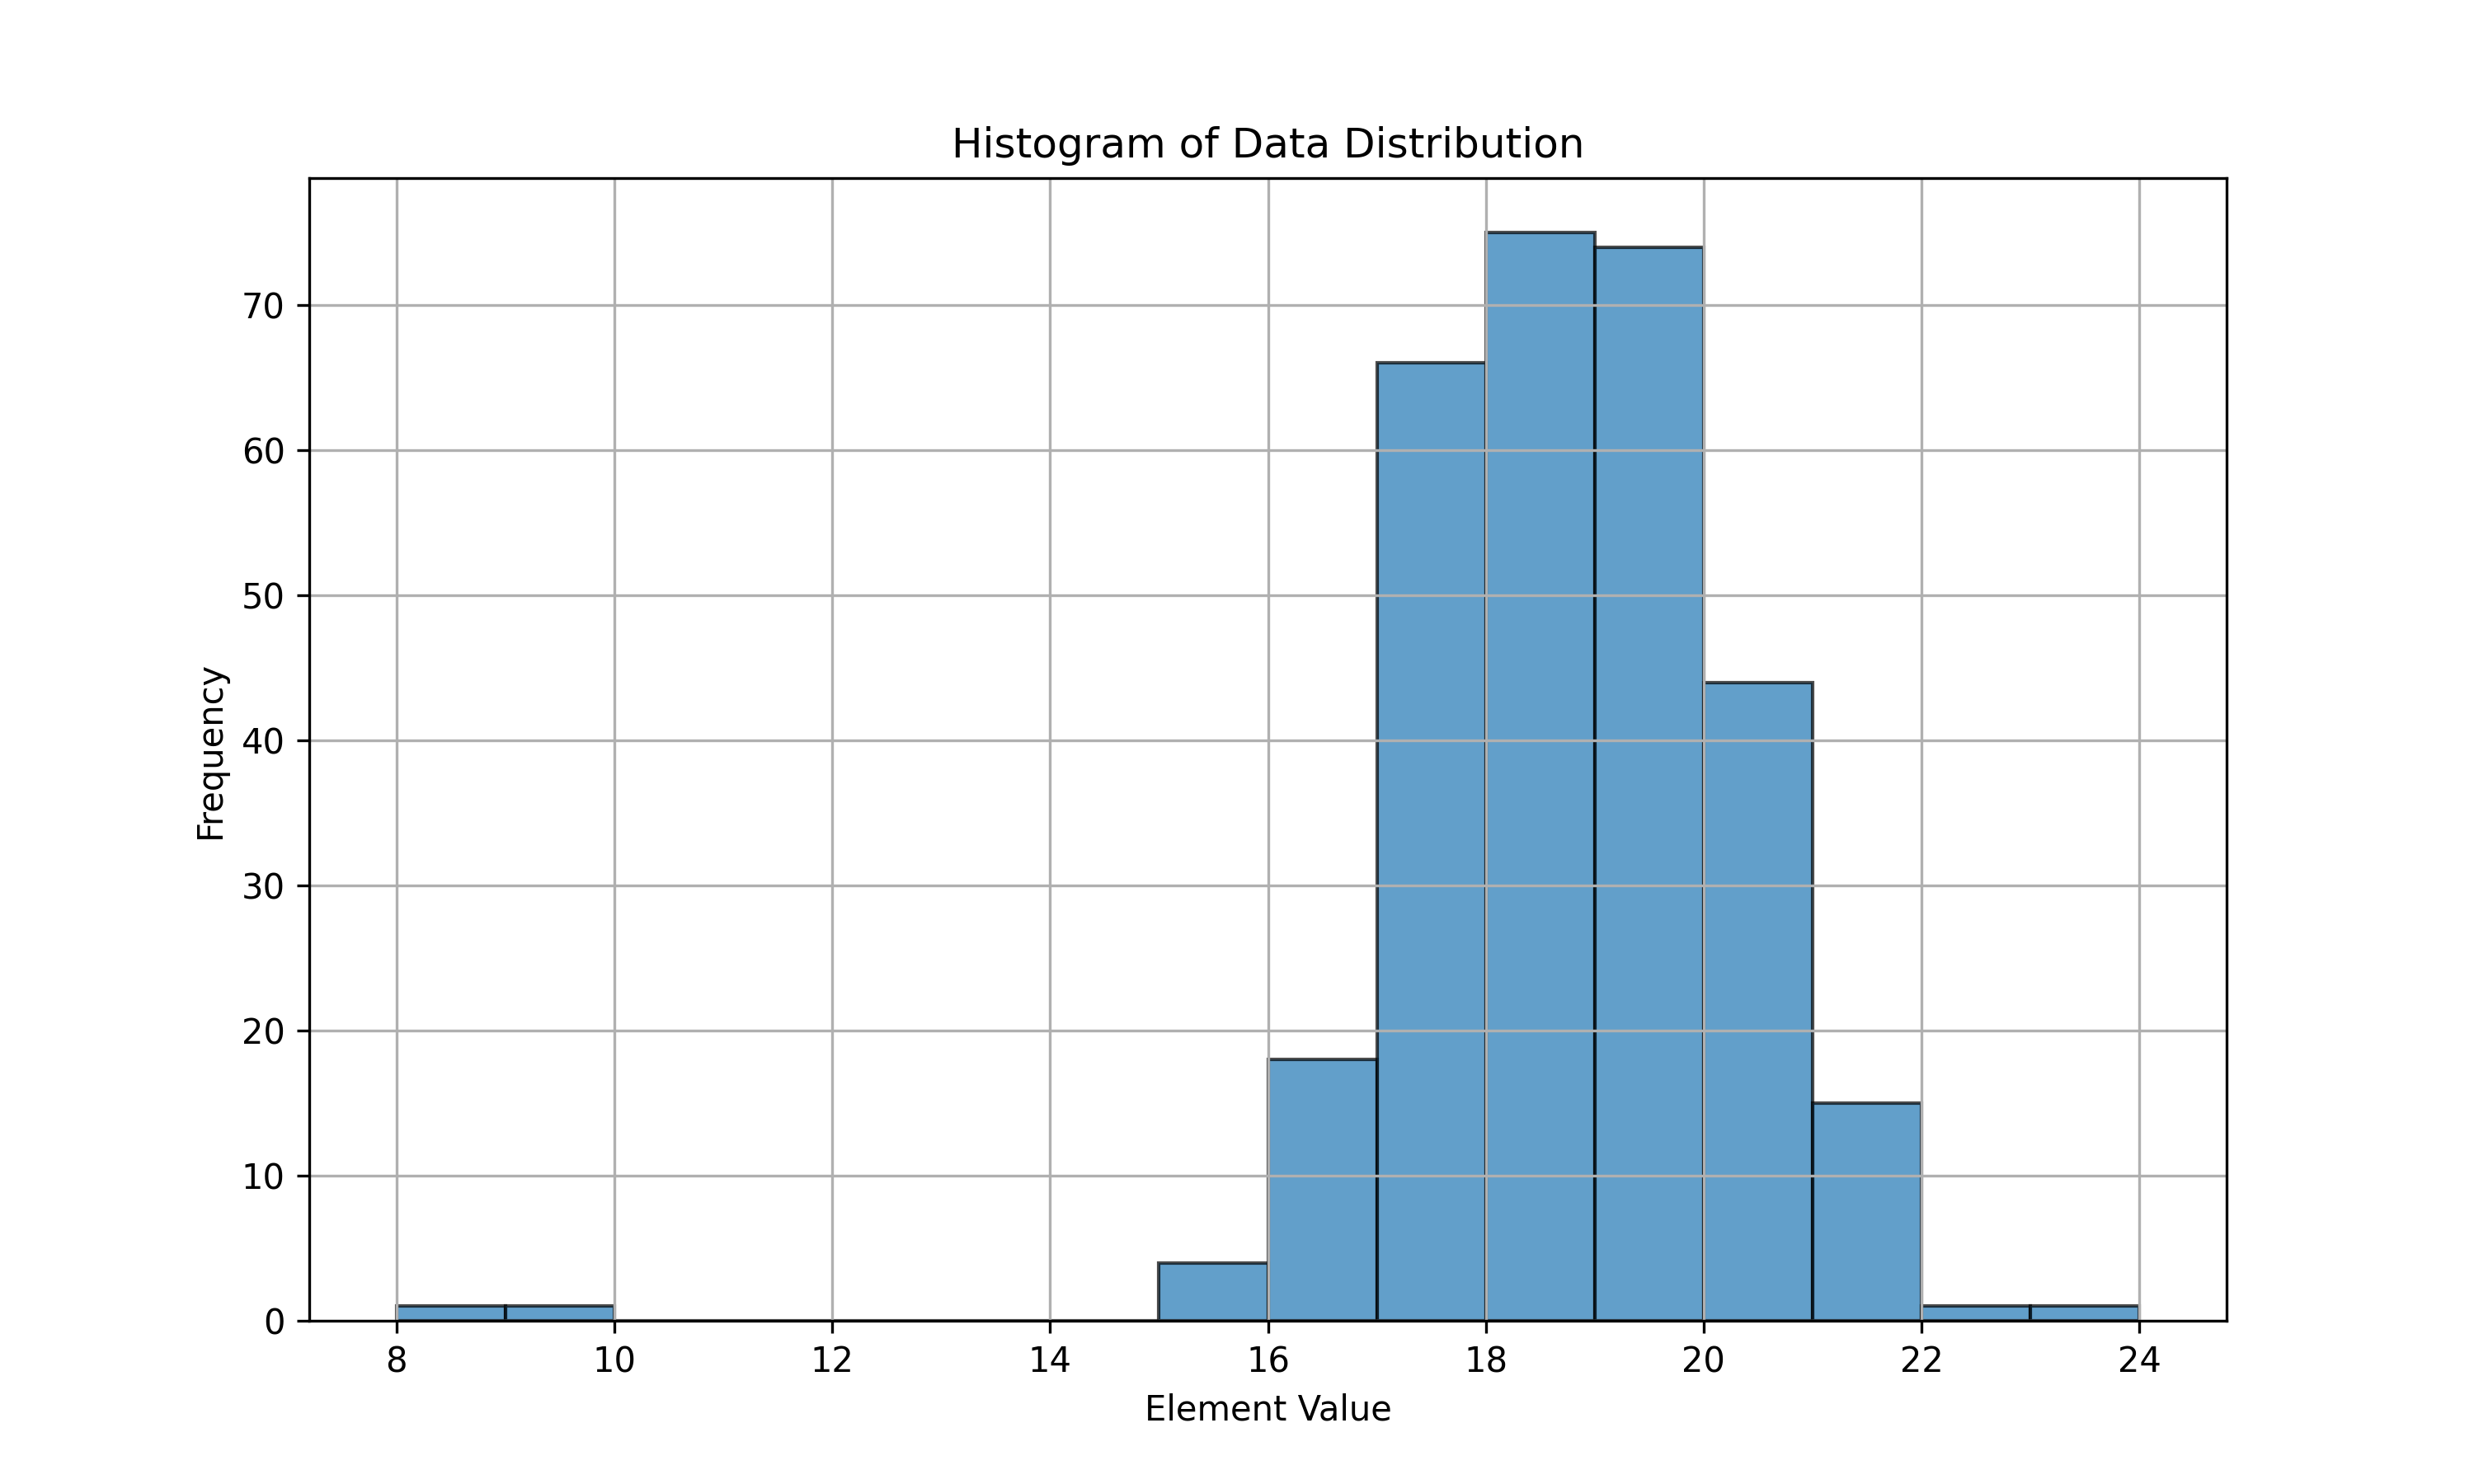
\includegraphics[width=1\textwidth]{Figs/plot.png}
\end{center}
\caption{Syllables per haiku from 300 outputs}
\label{fig:plot2}
\end{figure}

As we can see in Figure~\ref{fig:plot2}, the vast majority of generated haikus are between 17 and 19 sylalbles, with a few outliers.
These can be explained by either the model incorrectly counting syllables from words that are not
in the CMU Pronouncing Dictionary \citep{cmu_pronouncing_dictionary}, or the syllable counting algorithm
miscalculating the output.
We are aiming to have our model only output 17 syllable haikus where possible - there are more methods we will be integrating into the model.

\textbf{Qualitative Results:} \\
The model generates a mix of interesting or funny hakius, and incoherent outputs:
\begin{itemize}
  \item \textit{“river flows wildly \\
  air patches on the surface \\
  dissipates in life”}
  \item \textit{“rainfall through the roof \\
  dancers from serenity \\
  as his life goes by”}
  \item \textit{“grass on the wayside \\
  looking for the light to come \\
  warm clouds and weather”}
  \item \textit{“bloom gives way to me \\
  for i am not your hero \\
  i am george carlin”}
  \item \textit{“pond ripples to steal \\
  winters for having their gaze \\
  beg for hope bears now”}
  \item \textit{“branch and wood filters \\
  of night bright and sunny day \\
  hot lemonade waits”}
  \item \textit{“stream sits and pure fish \\
  in between and i am glad \\
  with what we i”}
  \item \textit{“ancient tree freedom \\
  anxiety creation \\
  ignites and section”}
\end{itemize}

As we can see, the model is able to generate haikus that could pass for human-written, however, it still generates
incoherent haikus. Moving towards generating more coherent outputs will be a focus of ours as we improve to model.

The main challenges we faced making this model were
related to ensuring syllable structure and was maintained and the syllable counts were accurate, and
slow training times.

Because of irregularities in the English Language, we found it difficult to
come up with a reliable method to count the number of syllables in a given word. Our current solution involves referencing
the CMU Pronouncing Dictionary \citep{cmu_pronouncing_dictionary} to get the syllable count of a given word.
However, this method is not perfect, as the CMU Pronouncing Dictionary does not contain all words that may show up in our vocabulary.
This causes issues when a word is not in the dictionary, so we are looking to integrate algorithms that can help resolve this, although this still only provides an approximation which can lead to slight issues during generation.

The slow training times were due to the large amount of data and limited access to compute resources. We tested differing batch sizes to reach a reasonable training time given our resources, however we are looking into ways to gain access to more powerful GPUs to speed up training.

\label{last_page}

\bibliography{APS360_ref}
\bibliographystyle{iclr2022_conference}

\end{document}
